\chapter{Problem Statement}
HTTP/1.1 was first documented in RFC 2068 \cite{b9} and since its inception, it supports sending multiple HTTP requests over the same TCP or SSL/TLS socket. The HTTP requests are sent back to back and the server uses the HTTP headers to identify where a request ends and the subsequent request starts. \\
Consider an architecture composed of a chain of systems as depicted in \ref{fig:HTTP Desync Attack}

\begin{figure}
	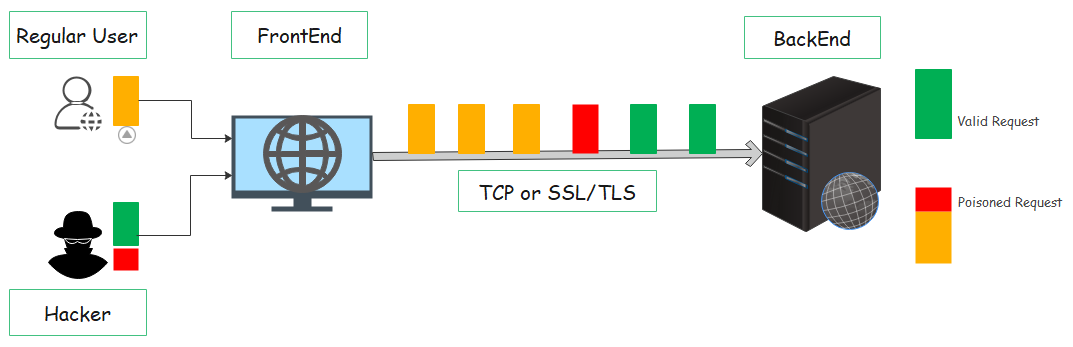
\includegraphics[width=14cm]{images/HTTP_Desync}
	\caption{HTTP Desync Attack}
	\label{fig:HTTP Desync Attack}
\end{figure}